\chapter{Anexos}
\label{chap:anexos}


\section{Proyecto de una red de monitoreo continuo de CL en la Ciudad de México}}

\newpage

\section{Proyecto \textit{International Dark Sky Place} en el Geoparque Comarca Minera}

El programa \textit{International Dark Sky Place} de la \textit{International Dark-Sky Association} (IDA) fue fundado en 2001 para incentivar a comunidades, parques y áreas protegidas localizadas alrededor del mundo para preservar y proteger los sitios con cielos oscuros a través de políticas de iluminación responsable y educación pública.\\

El programa ofrece seis tipos de designaciones entre las que se encuentra la \textit{International Dark Sky Park} (IDSP). Esta designación se refiere a lugares que poseen una distinguida calidad de noches estrelladas; un ambiente nocturno que está específicamente protegido por su patrimonio científico, natural, educativo, cultural y/o disfrute público.\\

Actualmente existen 76 IDSPs certificados por el IDA en países como Estados Unidos, España, Japón, Inglaterra y Canadá, pero ninguno en México ni América Latina.\\

En sinergia con Carles Canet, Secretario Académico del Centro de Ciencias de la Atmósfera de la Universidad Nacional Autónoma de México y Coordinador de la Red de Geoparques de América Latina y el Caribe, se propone el geositio Peña del Aire perteneciente al Geoparque Comarca Minera para ser inscrito en el programa IDSP.\\

Peña del Aire es un mirador paisajístico gestionado por el Ejido de San Sebastián, que se encuentra en el municipio de Huasca de Ocampo, Hidalgo; forma parte de la Reserva de la Biósfera de la Barranca de Metztilán y está ubicado a 100 km de la Ciudad de México, y a 30 km de Pachuca.\\

Los requerimientos mínimos de elegibilidad de un sitio para su inscripción en el programa IDSP son: 

\begin{itemize}

	\item Crear un plan integral de gestión de la iluminación

    \item Cumplir con condiciones nocturnas típicas como la visibilidad de la Vía Láctea a simple vista
    
    \item Demostrar el compromiso con los cielos oscuros a través de la elaboración de documentos educativos, inventarios de iluminación y un programa continuo de monitoreo de contaminación lumínica
    
     \item Presentar evidencia de liderazgo por parte del parque al colaborar con otras instituciones en proyectos de restauración de los cielos oscuros
     
     \item Elaborar programas de divulgación científica acerca de la importancia de los cielos oscuros y los beneficios de la correcta iluminación
    
\end{itemize}

Los beneficios de una designación IDSP son el reconocimiento internacional de los programas y actividades del parque para proteger los cielos oscuros y la autorización para el uso del logotipo de la IDA en publicaciones y grupos comerciales. Por su parte, la IDA promoverá los esfuerzos del parque a través de su página web y redes sociales.\\

La información presentada referente al IDSP, así como la guía para la nominación y fechas de las aplicaciones anuales se encuentran en la página web de la IDA \url{darksky.org}.

\newpage

\section{Código en Julia del Mapa CL-CDMX}}

\lstinputlisting[language=Julia]{CodigoMuestra.jl}

\newpage

\section{Tendencias de radiancia en las alcaldías de la Ciudad de México}}

\begin{figure}[H]
  \centering
    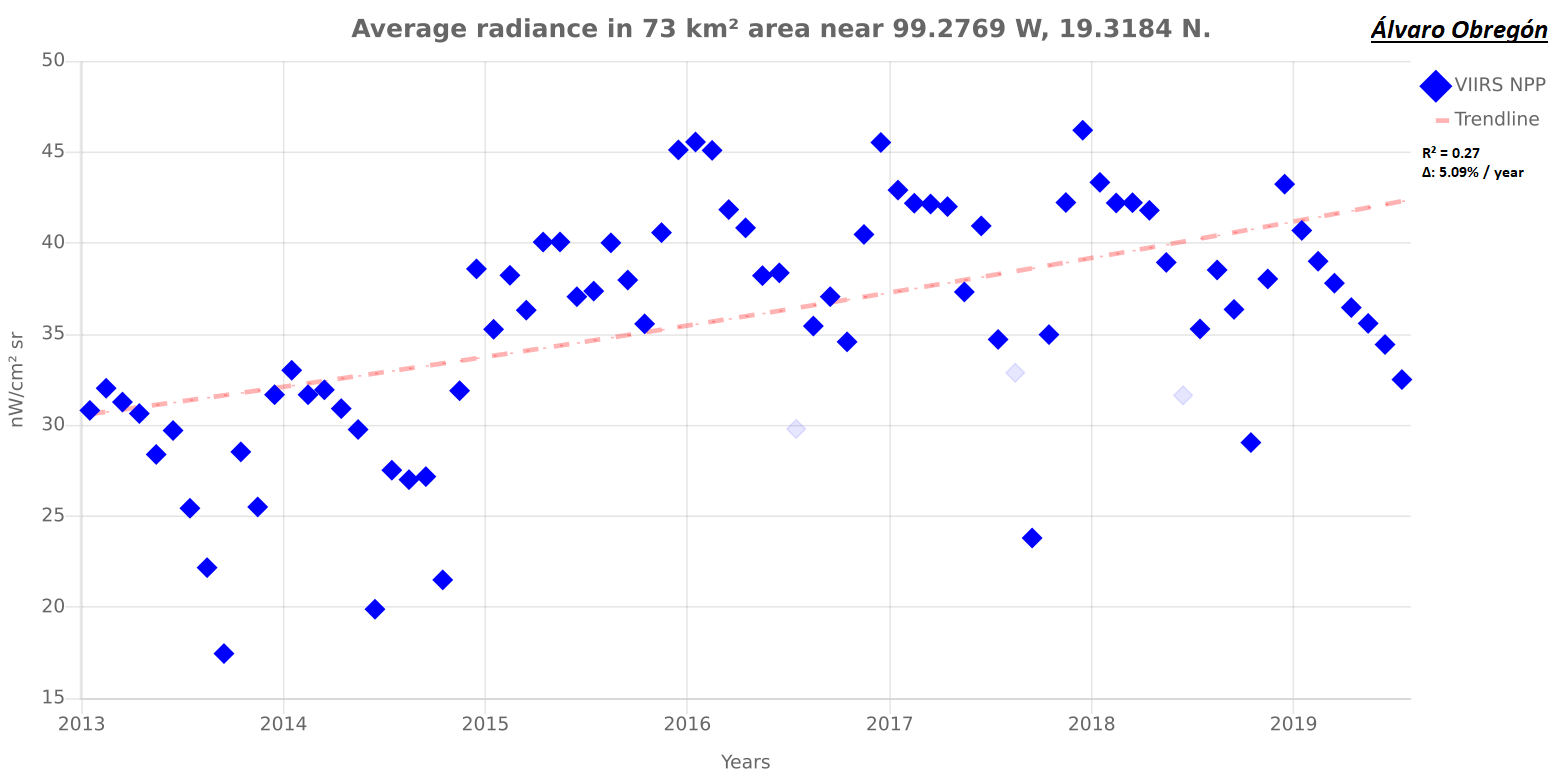
\includegraphics[width=1\textwidth]{AO}
  \caption{Tendencia de radiancia promedio para la alcaldía Álvaro Obregón}
  \label{radiancetrendsao}
\vspace{20mm} 
    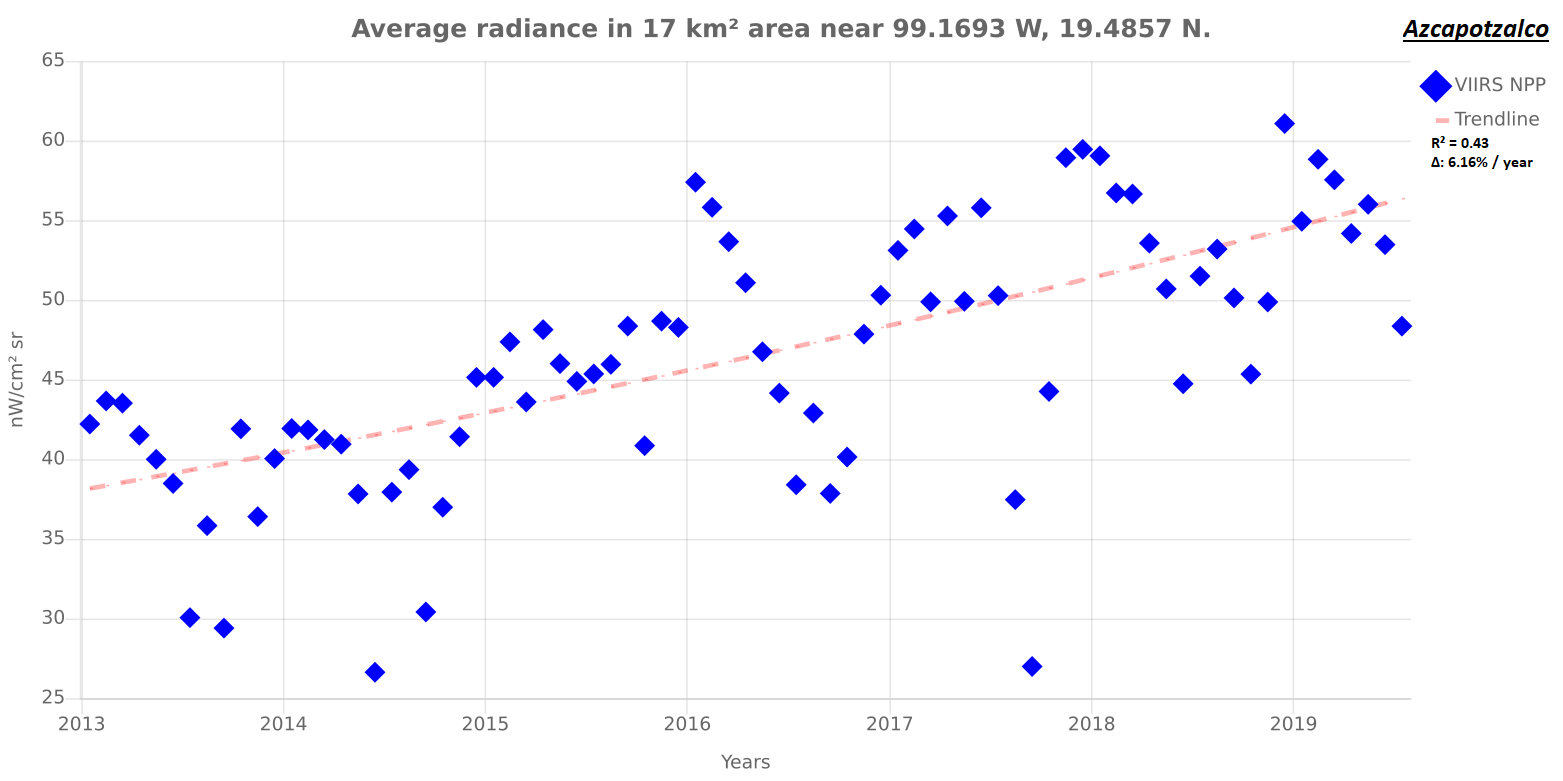
\includegraphics[width=1\textwidth]{AZ}
  \caption{Tendencia de radiancia promedio para la alcaldía Azcapotzalco}
  \label{radiancetrendsaz}
\end{figure}
\blindtext

\newpage

\begin{figure}[H]
  \centering
    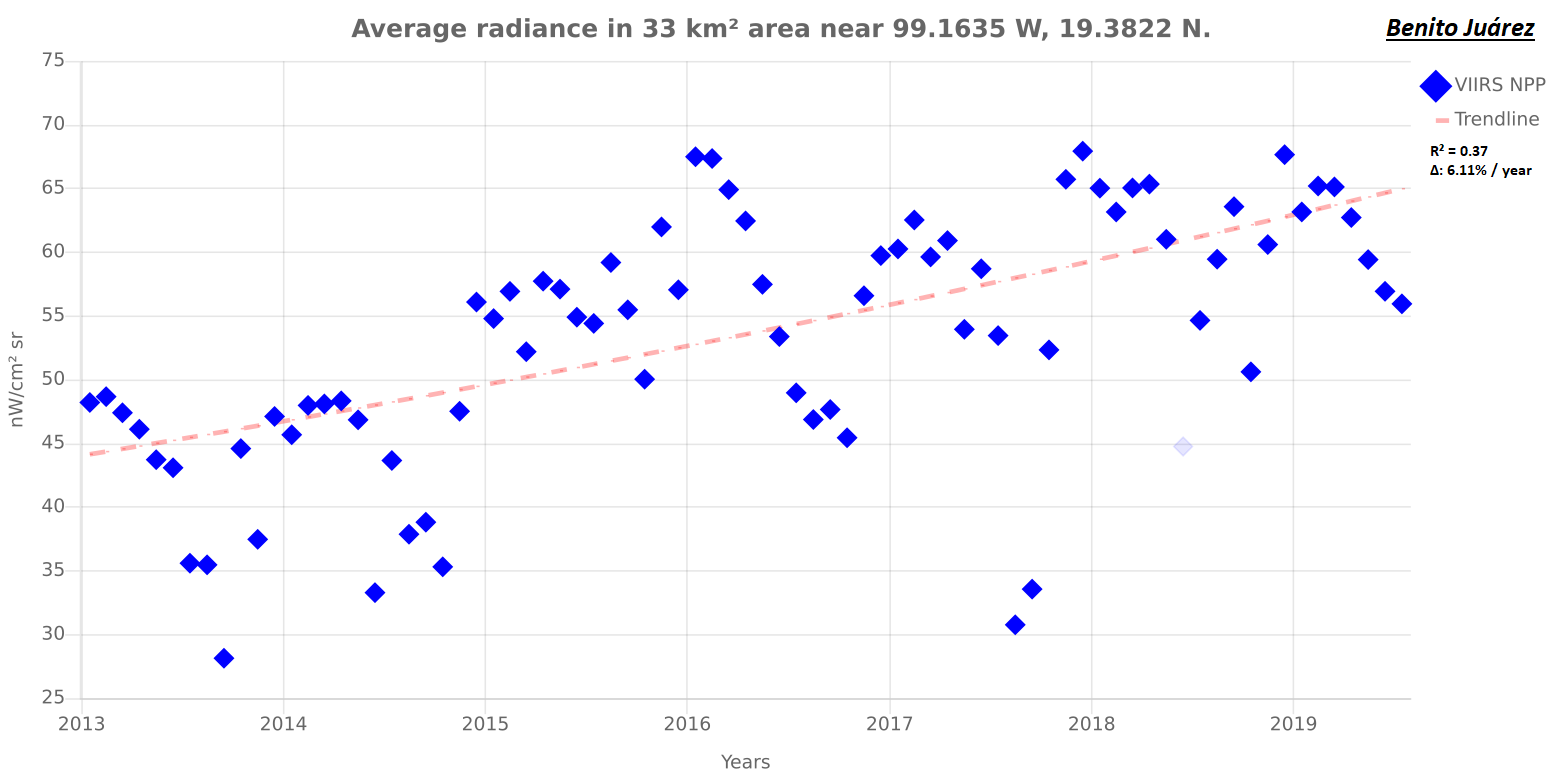
\includegraphics[width=1\textwidth]{BJ}
  \caption{Tendencia de radiancia promedio para la alcaldía Benito Juárez}
  \label{radiancetrendsbj}
\vspace{20mm} 
    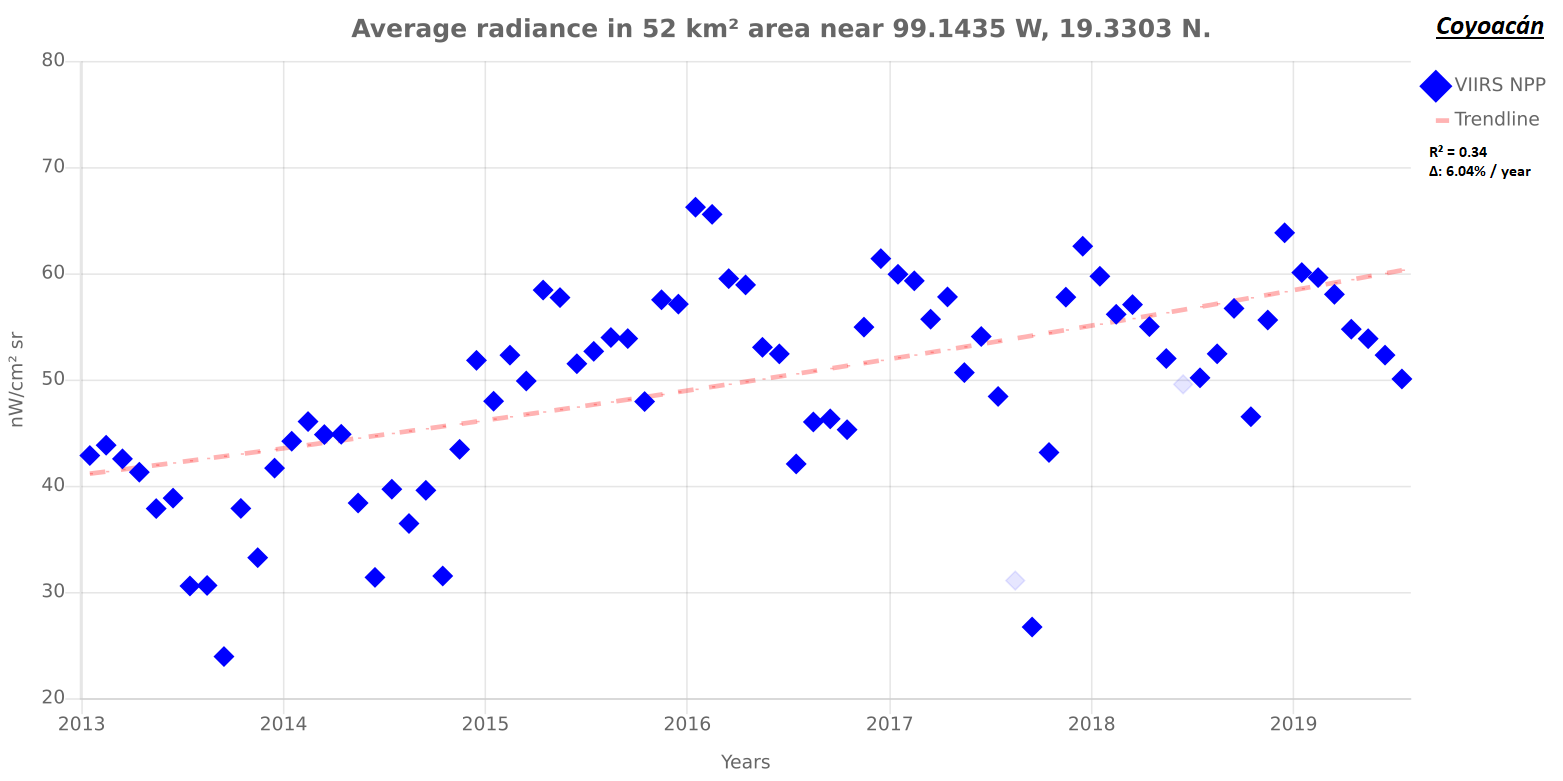
\includegraphics[width=1\textwidth]{CO}
  \caption{Tendencia de radiancia promedio para la alcaldía Coyoacán}
  \label{radiancetrendsco}
\end{figure}
\blindtext

\newpage

\begin{figure}[H]
  \centering
    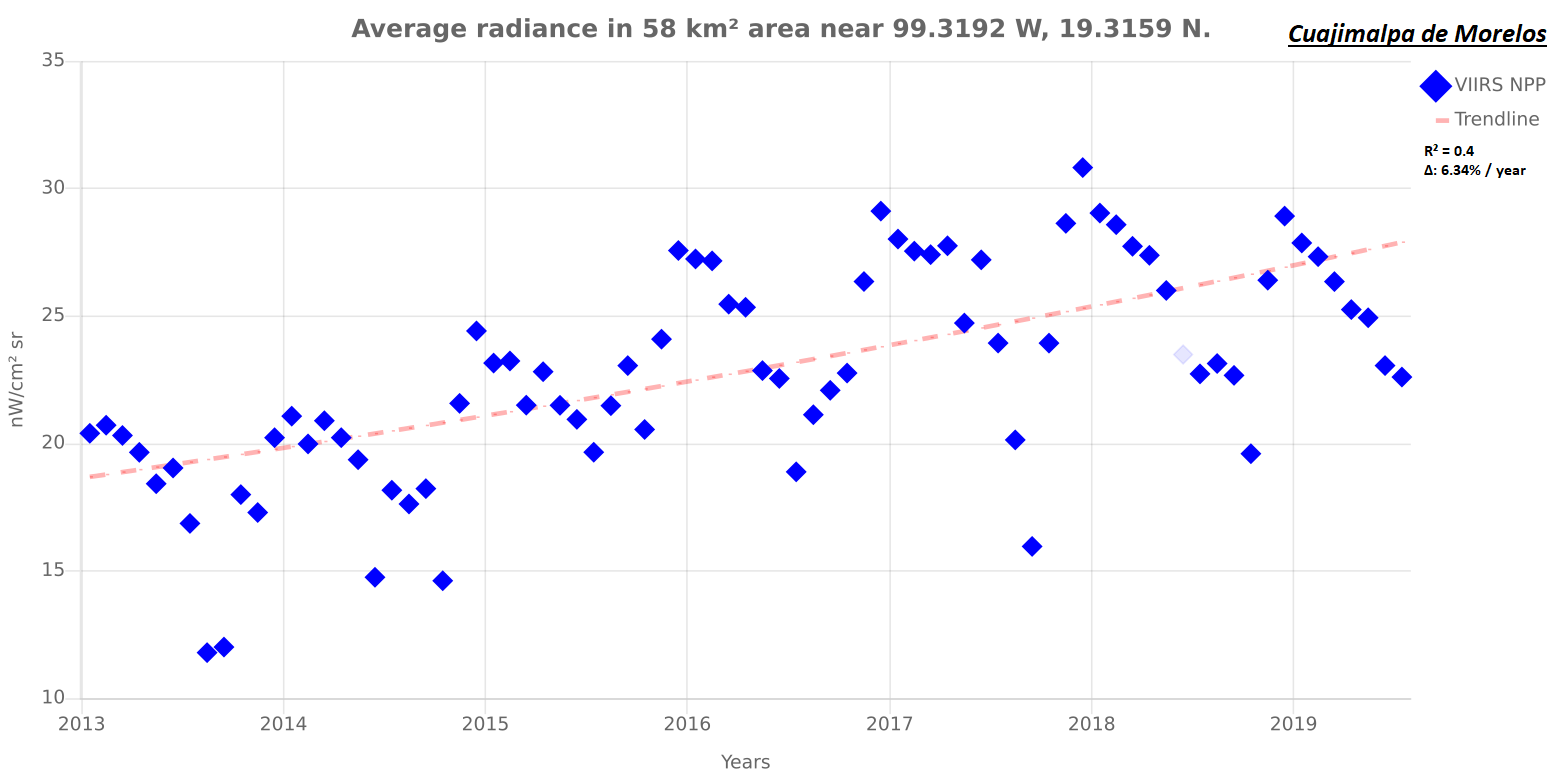
\includegraphics[width=1\textwidth]{CM}
  \caption{Tendencia de radiancia promedio para la alcaldía Cuajimalpa de Morelos}
  \label{radiancetrendscm}
\vspace{20mm} 
    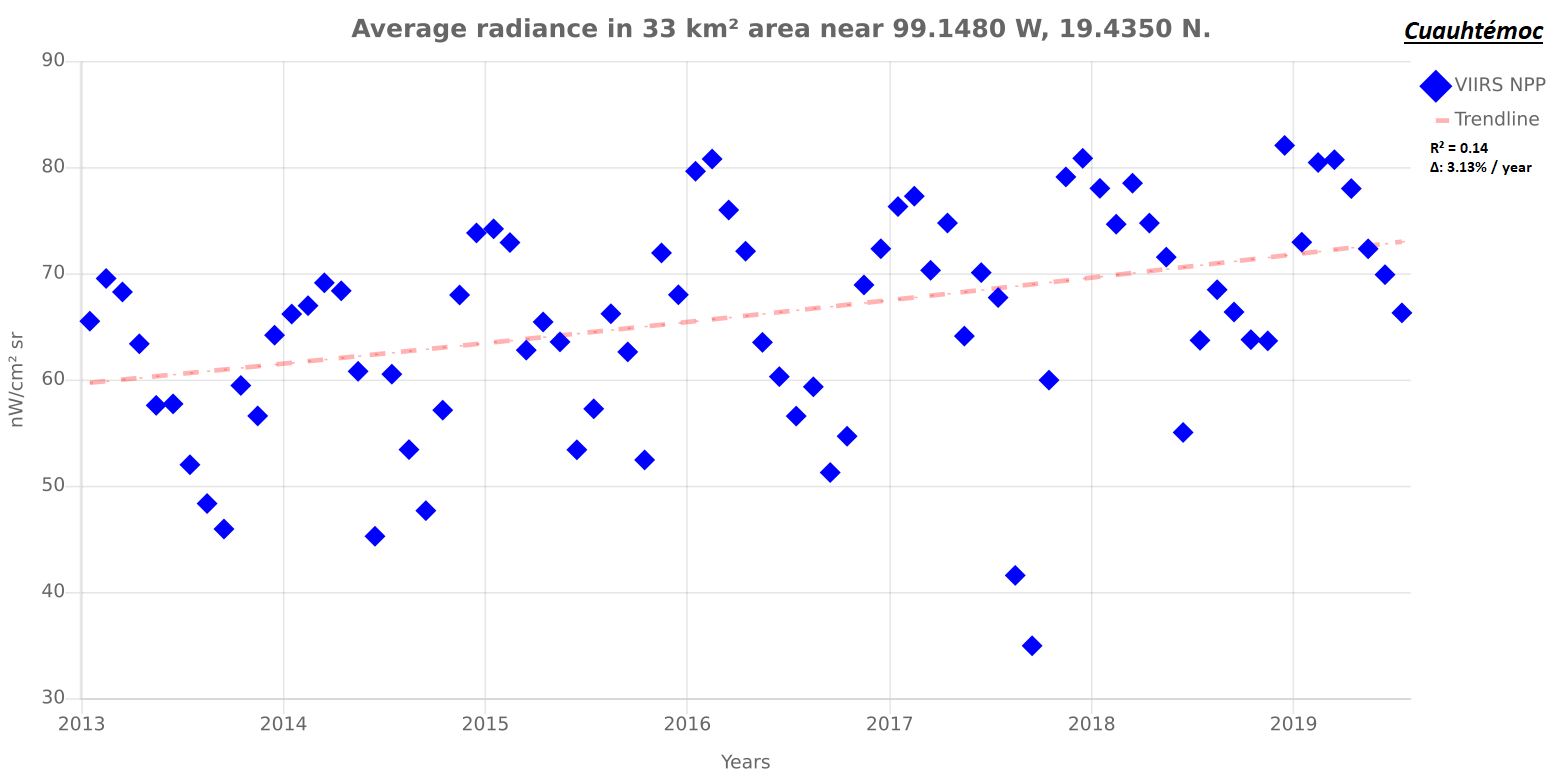
\includegraphics[width=1\textwidth]{CUA}
  \caption{Tendencia de radiancia promedio para la alcaldía Cuauhtémoc}
  \label{radiancetrendscua}
\end{figure}
\blindtext

\newpage

\begin{figure}[H]
  \centering
    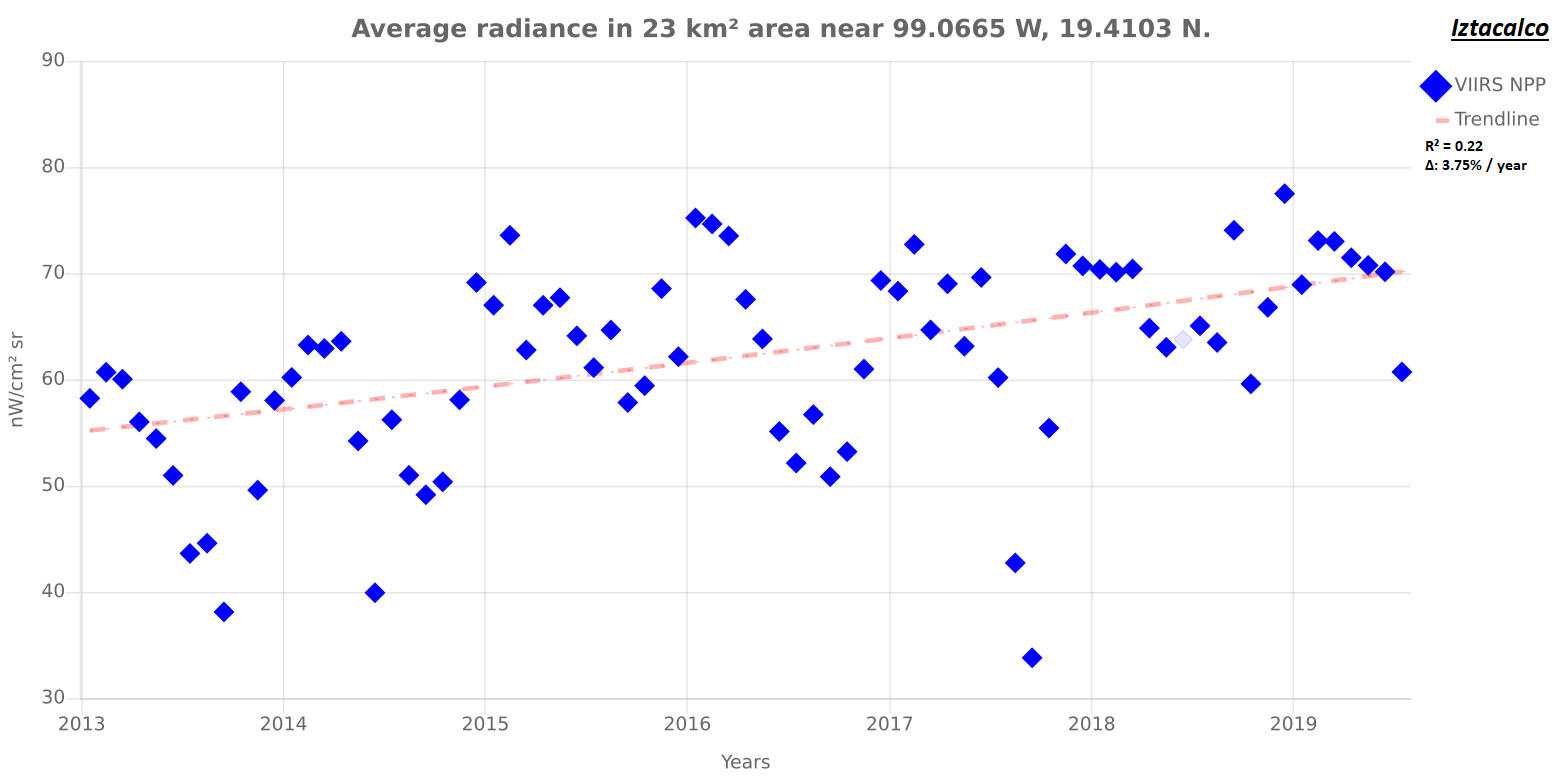
\includegraphics[width=1\textwidth]{IZT}
  \caption{Tendencia de radiancia promedio para la alcaldía Iztacalco}
  \label{radiancetrendsizt}
\vspace{20mm} 
    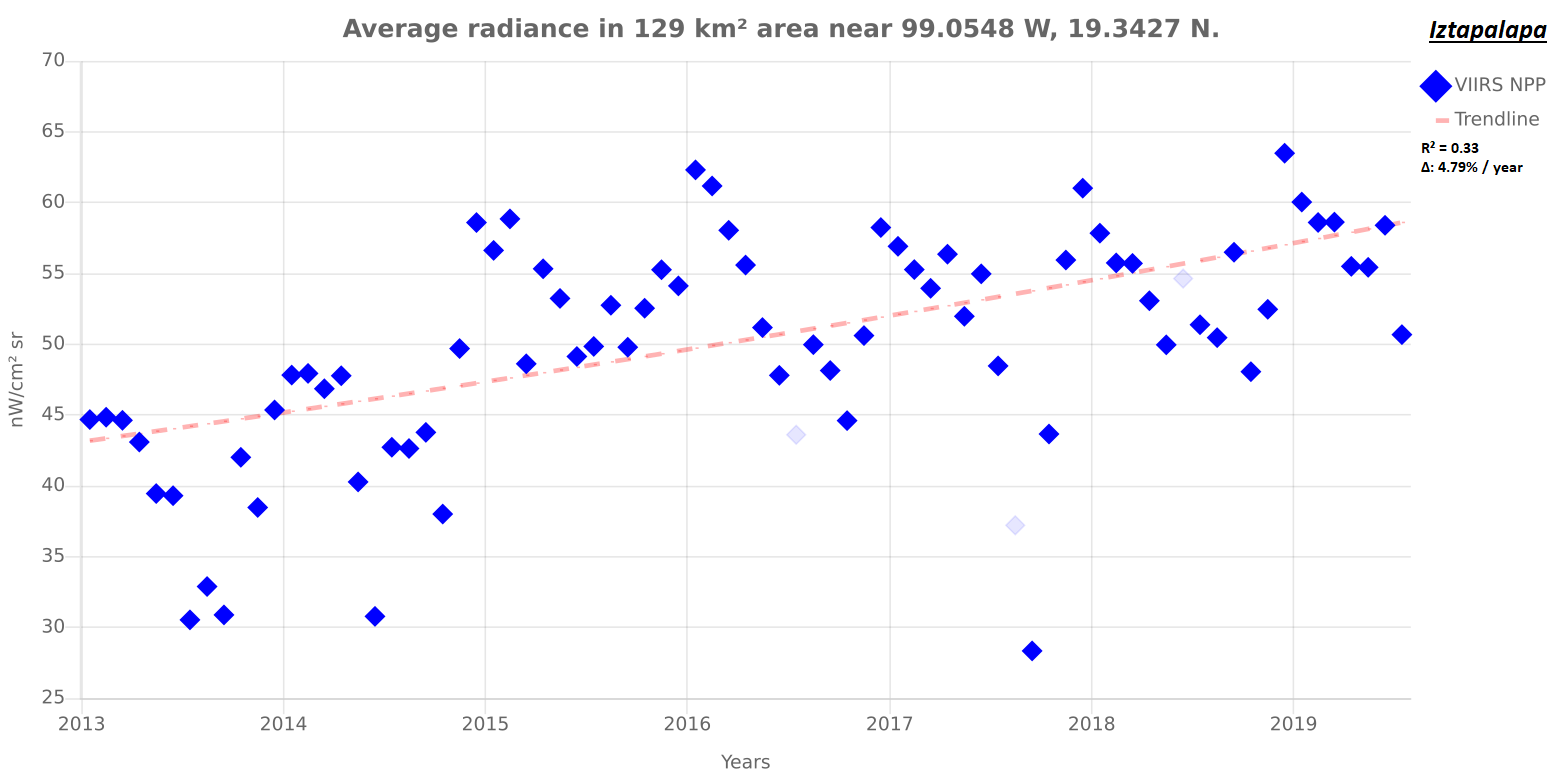
\includegraphics[width=1\textwidth]{IZP}
  \caption{Tendencia de radiancia promedio para la alcaldía Iztapalapa}
  \label{radiancetrendsizp}
\end{figure}
\blindtext

\newpage

\begin{figure}[H]
  \centering
    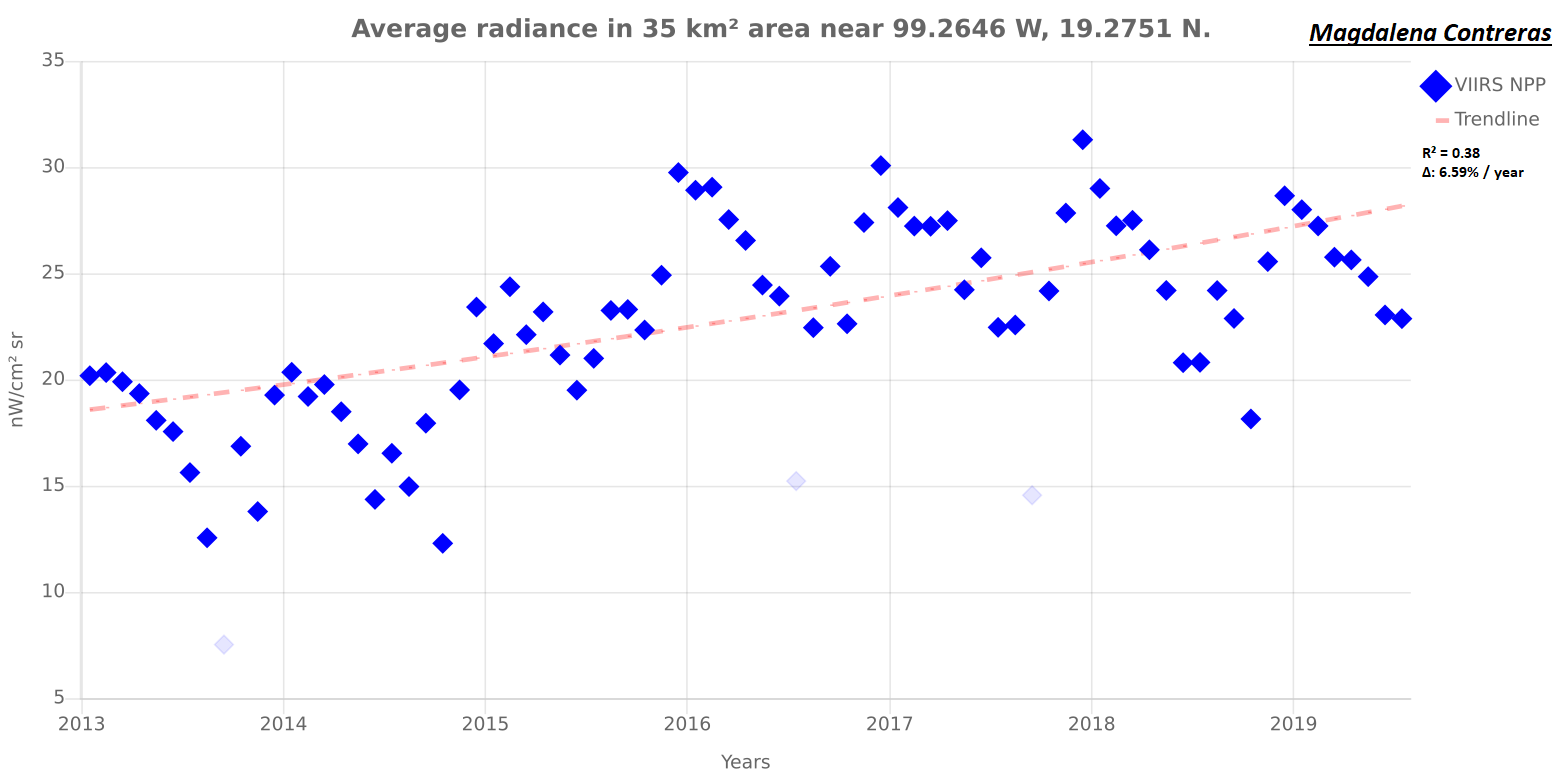
\includegraphics[width=1\textwidth]{MC}
  \caption{Tendencia de radiancia promedio para la alcaldía Magdalena Contreras}
  \label{radiancetrendsmc}
\vspace{20mm} 
    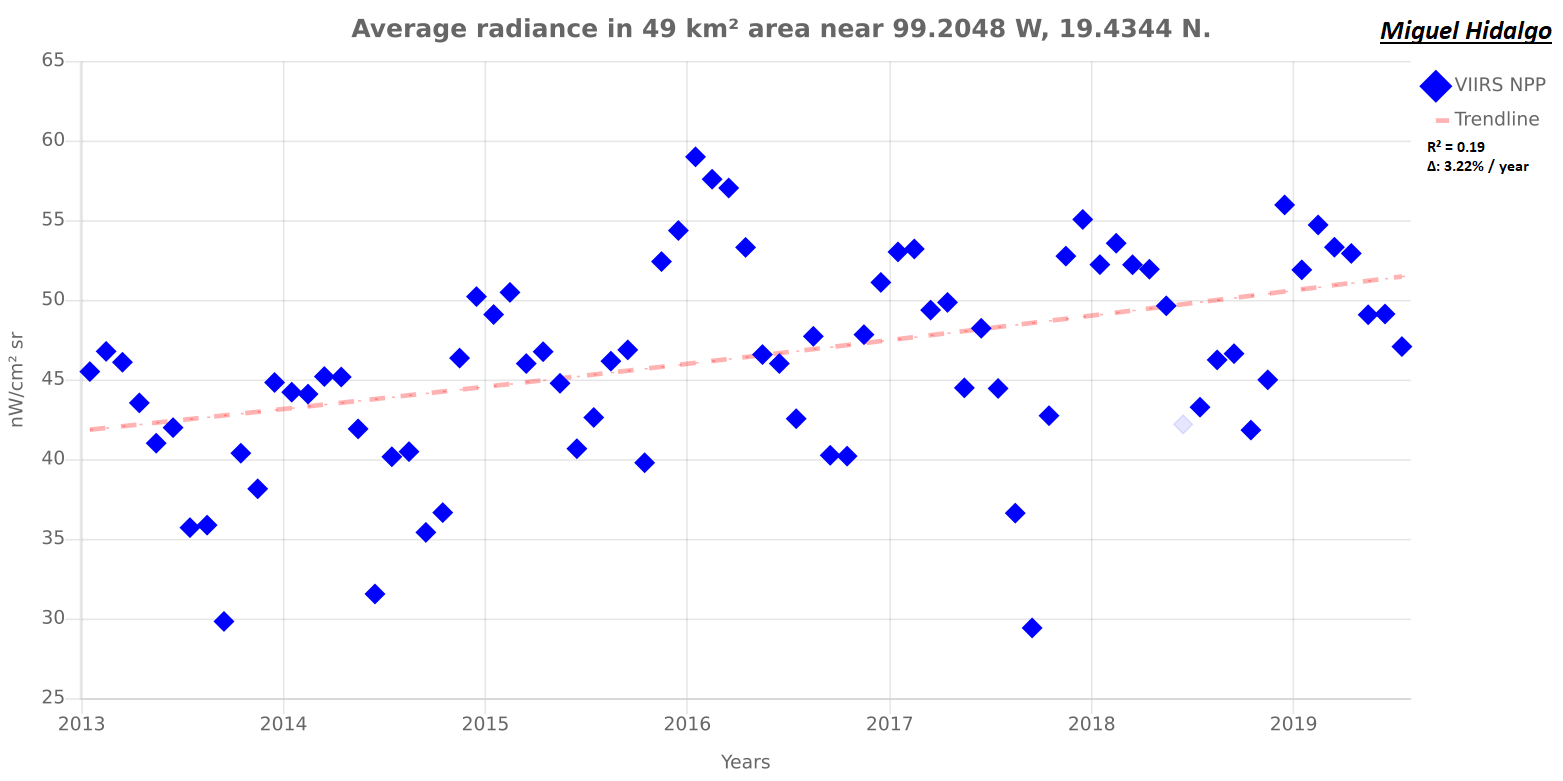
\includegraphics[width=1\textwidth]{MH}
  \caption{Tendencia de radiancia promedio para la alcaldía Miguel Hidalgo}
  \label{radiancetrendsmh}
\end{figure}
\blindtext

\

\begin{figure}[H]
  \centering
    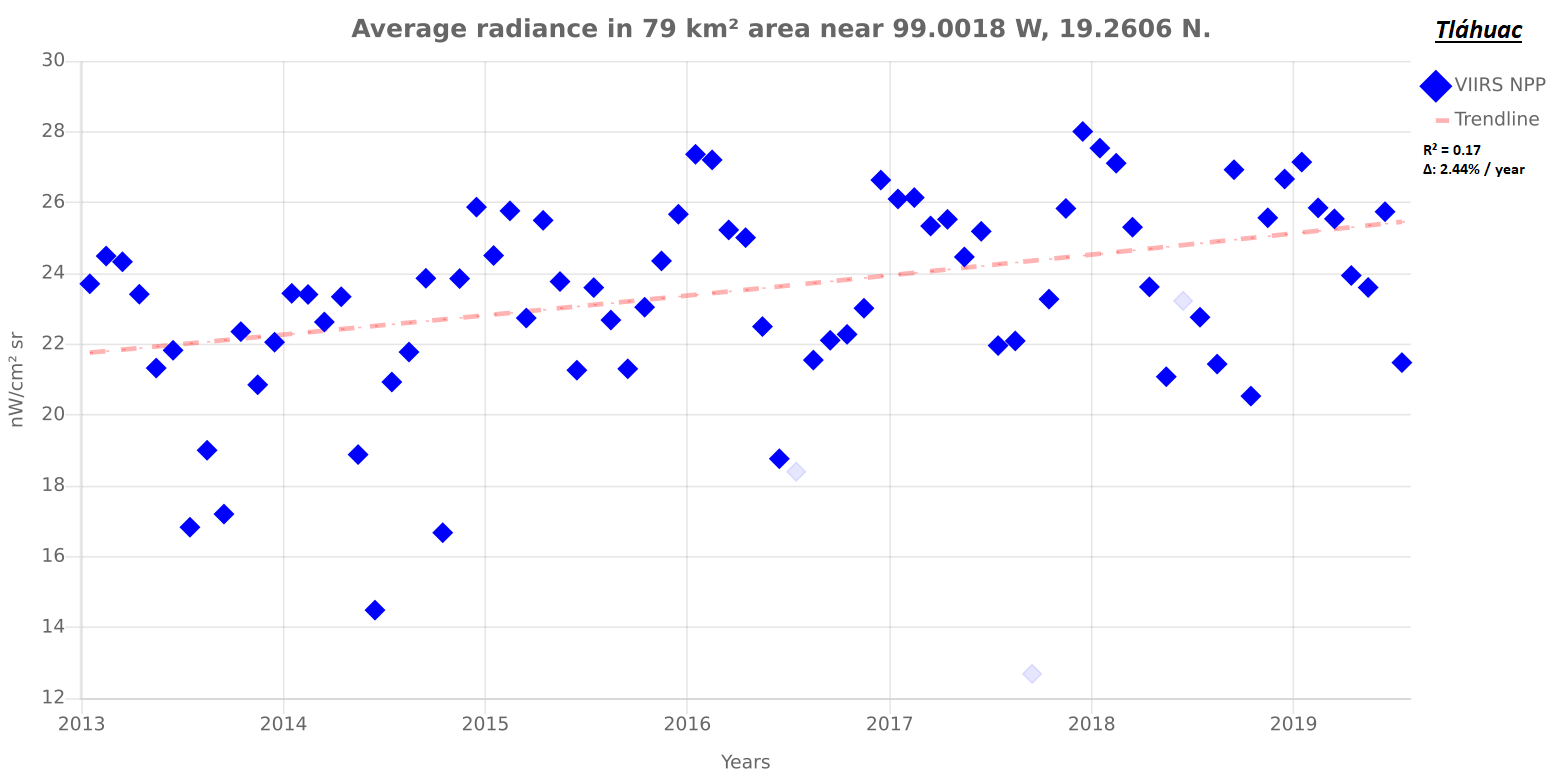
\includegraphics[width=1\textwidth]{TLAH}
  \caption{Tendencia de radiancia promedio para la alcaldía Tláhuac}
  \label{radiancetrendstlah}
\vspace{20mm} 
    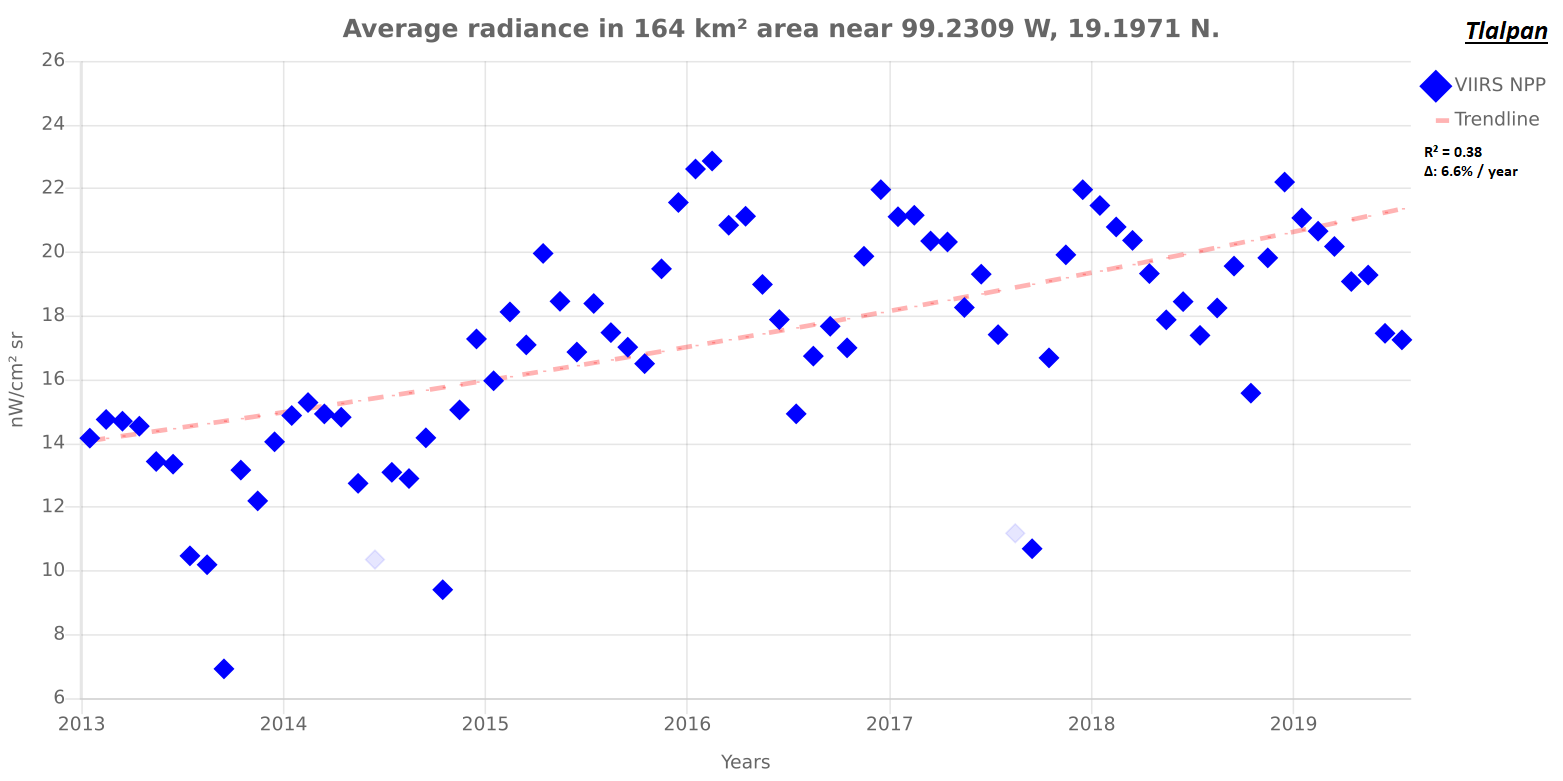
\includegraphics[width=1\textwidth]{TLA}
  \caption{Tendencia de radiancia promedio para la alcaldía Tlalpan}
  \label{radiancetrendstla}
\end{figure}
\blindtext

\newpage

\begin{figure}[H]
  \centering
    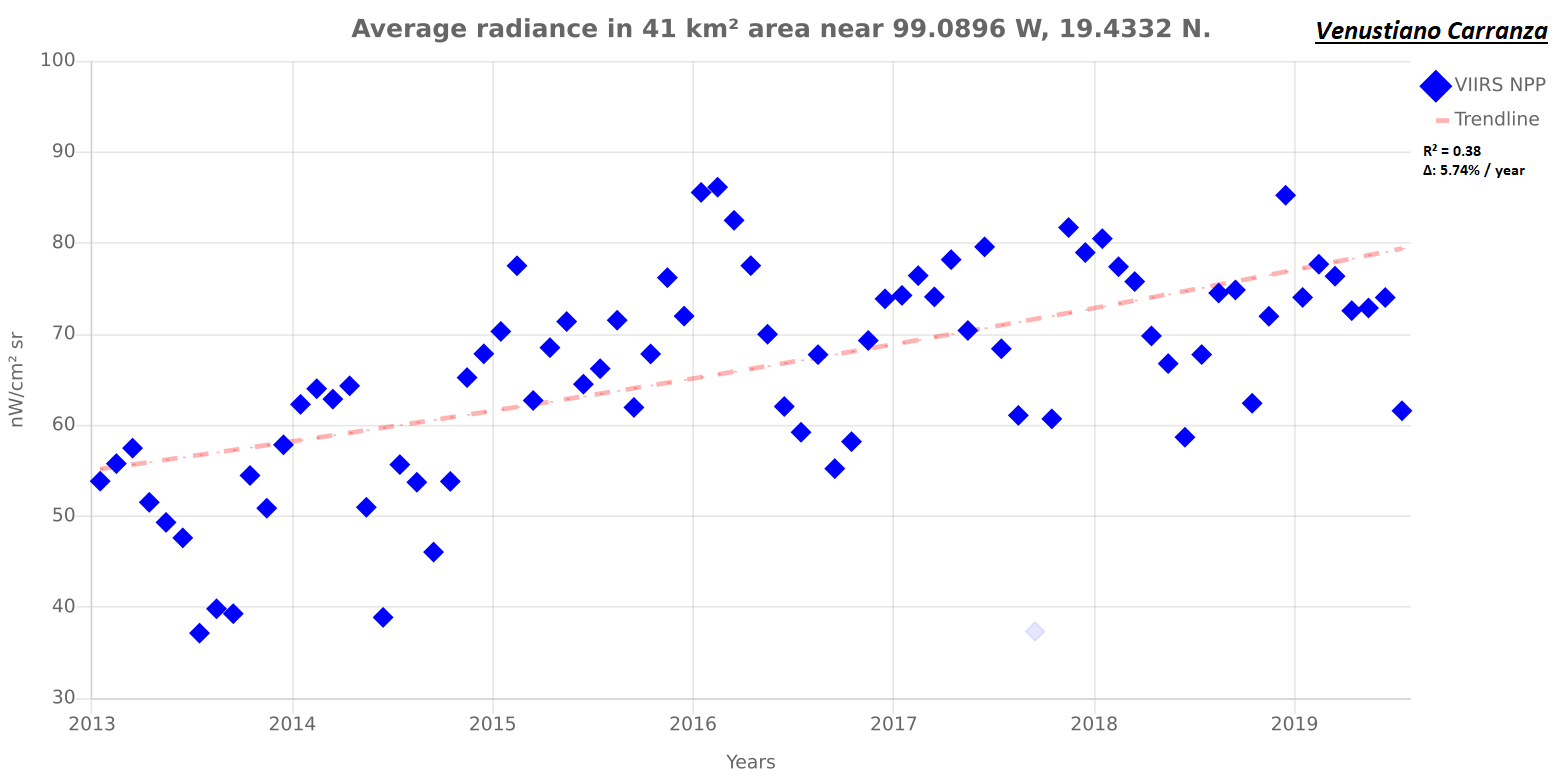
\includegraphics[width=1\textwidth]{VC}
  \caption{Tendencia de radiancia promedio para la alcaldía Venustiano Carranza}
  \label{radiancetrendstlah}
\vspace{20mm} 
    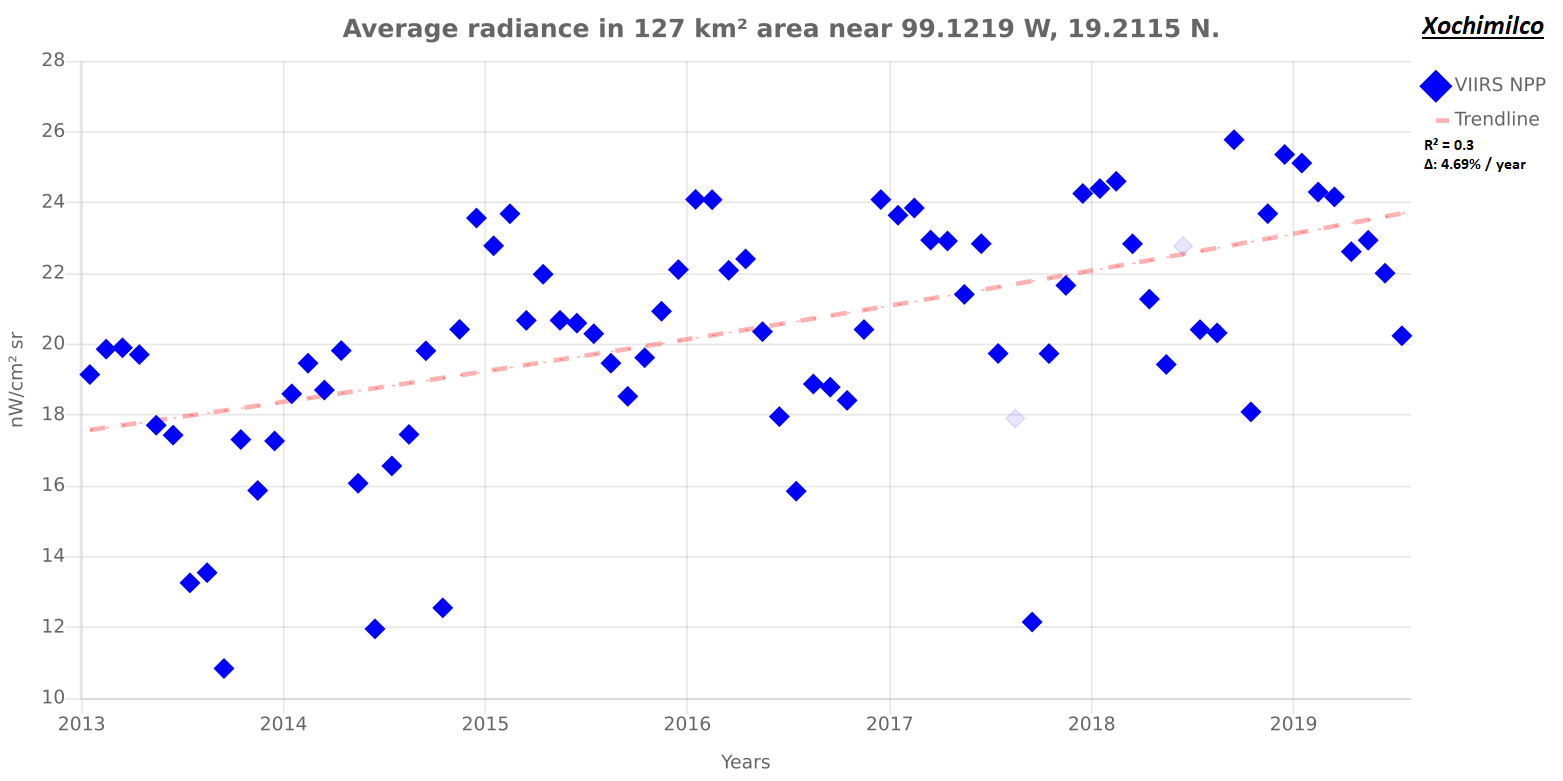
\includegraphics[width=1\textwidth]{XO}
  \caption{Tendencia de radiancia promedio para la alcaldía Xochimilco}
  \label{radiancetrendstla}
\end{figure}
\blindtext

\newpage